% WĄTPLIWOŚCI JĘZYKOWE oznaczone przez %?? !! oznacza miejsce, gdzie
% skończyłem ostatnio poprawiać

% przykłady w sieci value of <> [directly] represents the <>

% jak się pisze 16ms czy 16 ms

% argumenty funkcji są an, gdy piszemy ogólnie o działaniu tych
% funkcji

\documentclass[oneside,a4paper]{article}
\usepackage[sectionbib,bibnewpage]{apacite}
\usepackage{amsmath}
\usepackage{bm}
\usepackage{float}
\usepackage{graphicx}
\usepackage{listings}
\usepackage{caption}

\title{The bhsdtr package: a general purpose method of bayesian
  inference for Signal Detection Theory models}

\begin{document}
\maketitle
\tableofcontents{}

\section{Abstract}

We describe a novel method of bayesian inference for hierarchical or
non-hierarchical equal variance normal Signal Detection Theory models
with one or more criteria. The method is implemented as an open-source
R package that uses the state-of-the-art platform Stan for sampling
from posterior distributions. Our method can accommodate binary
responses as well as additional ratings and an arbitrary number of
nested
% ?? WSZYSTKIE sdt parameters CAN be regressed, więc the
or crossed random grouping factors. The SDT parameters can be
regressed on additional predictors within the same model via
intermediate unconstrained parameters, and the model can be extended
by using automatically generated human-readable Stan code as a
% ?? czy to jest przypadek other -> bez przedimka?
template. In the paper we explain how our method improves on other
similar available methods, we give an overview of the package,
demonstrate the ease of use by providing a real-study data analysis
walk-through, and show that the model successfully recovers known
parameter values when fitted to simulated data.

\section{Introduction}

Many tasks used in psychology studies are essentially classification
tasks. For example, in a memory study participants may be required to
decide if a given test item is old or new, or, in a perceptual study,
an object may either be a letter or a digit. If a task requires
classification it is always possible that conclusions based on
% ? an ability mi tu nie pasuje
accuracy or percent correct are invalid because ability to
discriminate between stimulus classes (i.e., sensitivity) is
confounded with bias, which is a tendency to classify stimuli as
belonging to a particular class \cite{GreenSwets66}. In principle, any
effect that manifests itself in differences in classification accuracy
% ?? ani the sensitivity ani a sensitivity nie pasuje. Chodzi o
% ogólnie rozumiane zjawisko.
may reflect differences in sensitivity, bias, or both. Signal
Detection Theory provides a simple and popular solution to this common
and important problem.

However, because the SDT model is non-linear any variability in its
parameters due to factors such as participants or items has to be
accounted for, otherwise the estimates of SDT parameters are
biased. As we explain later in this paper, neither of the two
available methods of inference for hierarchical SDT models that we are
aware of addresses this problem correctly. Hence, our main goal was to
create a correct implementation of the general hierarchical linear
regression structure defined on SDT parameters. We argue that the
\texttt{bhsdtr} package for R \cite{rstatistical} provides exactly
such an implementation and we have made it publicly available at
% ?? tylko jeden, konkretny kod i zbiór danych, o którym czytelnik
% dopiero się dowiaduje, ale o którym nie będziemy więcej mówić, czyli
% the
https://github.com/boryspaulewicz/bhsdtr, together with the annotated
source code that was used to perform all the analyses and produce all
the figures presented in this paper.

% OPIS STRUKTURY ARTYKUŁU

In what follows, after introducing the most common version of the SDT
model, we describe its generalization which can accommodate data from
rating experiments. Next, we explain briefly why, if a method of
inference for SDT models were to be of general use in psychology
studies, it is essential that it was based on a model equipped with
the general hierarchical linear regression structure. The
\texttt{bhsdtr} package meets this requirement thanks to a novel
parametrization. We describe this novel parametrization in great
detail and we motivate it by explaining how the reliance on a
relatively standard parametrisation leads to problems in the two other
available implementations. We end the first part of this paper with a
formal definition of the model as implemented in \texttt{bhsdtr}. The
second part contains an overview of the package and a tutorial in
which we demonstrate how to use our method in practice. Before we go
any further, however, a note on terminology seems in order.

% SAMPLED FACTOR

In the context of hierarchical modelling factors such as participants,
items, or replications are often referred to as groups. In our opinion
this naming convention may be confusing; a single participant is both
a group and a member of some group, while at the same time the term
"group" is perhaps most strongly associated with study conditions, as
in "experimental group". In this paper we use the term "sampled
factor" instead, because, by virtue of being a new term, it is
unambiguous, and because it seems descriptively correct: the term
"sampled factor" captures all the essential properties of such
variables, i.e., a nominal scale, the fact that values are sampled
from a larger population and are usually not of direct interest, as in
"this is only a sample", and that conclusions
% ?? jeżeli już mamy jakąś analizę statystyczną, to zakładamy, w
% uproszczeniu, że target population jest określona
of statistical analysis are meant to apply to the whole population of
possible values.

\section{Equal variance normal Signal Detection Theory model with
  additional criteria}

According to Signal Detection Theory each stimulus in a classification
task gives rise, by some unspecified cognitive process, to an
unidimensional internal evidence value $s$ sampled from
% ?? stimulus już był wprowadzony, więc jego klasa jest (jakaś, ale)
% określona
a distribution that depends on the stimulus class. For historical
reasons the two stimulus classes are often referred to as "noise" and
"signal", and task performance is described in terms of hits, correct
rejections, omissions, and false alarms, but this terminology is
appropriate only when the model is applied to tasks that require
detection, which is by far not always the case. In the most widely
used version of the model, shown in Fig.~\ref{basicsdt}, the two
evidence distributions are normal with the same variance, which is
usually fixed at unity to make the model identifiable. The distance
$d'$ between the means of the
% ?? sensitivity bez przedimka?
evidence distributions represents sensitivity. Because normal
distributions are unbounded, $s$ is always ambiguous, and so a
criterion $c$ placed on the evidence axis has to be used to reach a
discrete
% ?? bias bez przedimka?
decision. A participant is assumed to decide that a stimulus belongs
to the first class (e.g., an old item) if $s < c$, or that it belongs
to the second class (e.g., a new item) if $s \geq c$. The location of
the decision criterion $c$ represents bias.


\begin{figure}[H]
  \centering
  \includegraphics[width=.8\linewidth]{plot_basicsdt.pdf}
  \caption{Equal variance normal Signal Detection Theory model}
  \label{basicsdt}
\end{figure}

% Najprostsze użycie

Perhaps the simplest way of using this model is to fit it to observed
response counts and use the estimated $d'$ values in place of the
percent correct scores; If the model is correct, the resulting
performance measure is not contaminated by bias. Obviously, the model
may not be correct, which is one of the reasons why we focus more on
the generalized version shown in Fig.~\ref{sdtr} below.

% Model K >= 2

\begin{figure}[H]
  \centering
  \includegraphics[width=.8\linewidth]{plot_sdtr.pdf}
  \caption{Equal variance normal Signal Detection Theory model with
    additional criteria}
  \label{sdtr}
\end{figure}

This
% ?? applicable to czy applicable in
generalized model is applicable to studies where participants are
asked to rate their binary classification decisions on confidence or
some other performance or stimulus related
% the ratings, bo study już określone, podobnie jak (rodzaj)
% klasyfikacji binarnej, ale czy the ratings and THE binary ...?
dimension. The ratings and the binary classification decisions can be
provided together (e.g., "I am almost certain that it was a digit"),
or in an arbitrary order.

% MODELOWANIE RATINGÓW ZA POMOCĄ KRYTERIÓW

% ?? a combined response? Skoro mamy ratings (i w domyśle mamy też
% binary class.), to czy nie the combined response? A może
% jakiekolwiek ratingi są załatwione za pomocą (ogólnego rozwiązania)
% modelowania czegoś, co jest "odpowiedzią łączną"?
Ratings are accommodated by introducing additional criteria and
modelling a combined response $y$, which
% ?? znowu kwestia przedimków vs. and
represents both the binary classification decision and rating. The
value of $y$ increases with the strength of evidence in favor of the
second stimulus class. For example, if confidence is rated on a
four-point scale, then $y = 1$ when a subject decides
% ?? bodziec, który zobaczył badany, więc the? bo chodzi o decyzję o
% określonym dla decydenta bodźcu, a nie nieokreślonym dla decydenta?
that a stimulus belongs to the first class with certainty $4$, and
$y = 5$ when a subject decides that a stimulus belongs to the second
class with certainty $1$. More formally, if $K$ is the number of
possible combined responses then a subject is assumed to give response
$k$ if $s \in (\bm{c}_{k-1},\bm{c}_k]$, where $\bm{c}$ are the $K+1$
decision criteria, with $\bm{c}_0$ and $\bm{c}_K$ fixed at $-\infty$
and $+\infty$ respectively.

% UŻYWAĆ SDTR CHOĆBY PO TO, ŻEBY SPRAWDZIĆ JEGO ZAŁOŻENIA

There is a good reason to collect the ratings and use the generalized
SDT model from Fig.~\ref{sdtr} even when neither the ratings nor the
placement of criteria are relevant to the research problem.
% ?? If K = 2 to jakby: w (jakimś) przypadku, w którym, When K = 2 to
% jakby: zawsze, gdy ...? Czuję, że lepiej the data i the model potem
When $K = 2$ (no ratings), the SDT model fits perfectly, regardless of
it being a reasonably good approximation to reality or not, because
the data and the model have the same dimensionality. This makes the
generalization to the $K > 2$ case particularly important, as it is
% ?? niektóre lub wszystkie formal assumptions, ale mamy na myśli
% konkretny zbiór formal assumptions, który czytelnik już zna, a
% nawet, jeśli nie, to te założenia są unikalnie wyznaczone przed
% model - the?
only when $K > 2$, that the formal assumptions of the model (e.g.,
equal or unequal variance) can be tested\footnote{In contrast to the
  formal assumptions, a psychological interpretation of the SDT
  parameters can be tested even when ratings are not available, e.g.,
  by means of selective influence \cite{sternberg2001separate}}, which
is often done by comparing observed and predicted ROC curves.

When SDT models are used in psychology studies, researchers are
usually interested in relationships between SDT parameters and
additional measured or manipulated
% ?? the dependence, bo ogólnie rozumiana kwestia zależności, stimulus
% strength - ogólne zjawisko, a nie jakaś konkretna, albo pojedyncza,
% ale bliżej nieokreślona
variables; A good example is the dependence of $d'$ on stimulus
strength. Also, in a great majority of psychology studies in which
classification tasks are used the data have hierarchical structure,
i.e., there are repeated measures for each participant or item and
participants or items are only samples from the target population. It
seems worthwhile to explain why a general-purpose method of inference
for SDT models should accommodate both kinds of situations.

% ?? Ważność hierarchical structure jako takiej
\subsection{The importance of hierarchical regression structure}

If data have hierarchical structure, but variability due to subjects,
items, or other sampled factors is not accounted for, estimates of
average (fixed) effects are not guaranteed to be unbiased and
conclusions are not guaranteed to generalize to a target population. A
not so uncommon practice of analysing data aggregated over sampled
factors represents an extreme case of ignoring
% ?? nieokreślona hier. structure, bo tu mówimy o externe case
% ogólnego zjawiska ignorowania ogólnej kwestii hierarchiczności
hierarchical data structure. Invalidity of this approach in the
% ?? Jeżeli illustrated w czasie przeszłym dokonanym i mówimy zaraz
% czyje rezultaty, to chyba the results?
context of SDT was clearly illustrated with the results of
simulational studies by \citeA{morey2008problematic}, although,
strictly speaking, it requires such demonstrations only in order to
make a point about a specific case. Because SDT is a non-linear model,
% ?? data jest unikalne dla tokenów estimates, więc the data?
by definition, when estimates of its parameters are based on data
aggregated over sampled factors the expected values of these estimates
are not in general true population averages. Such estimates are
% ?? zakładamy (w uproszczeniu), że target population jest ustalona
% dla każdego estimate
biased and inference about a target population based on such estimates
is simply not valid. To give a concrete example, consider two unbiased
participants, one with $d'_1 = 2$ and one with $d'_2 = 4$. Their
expected average accuracy is given by
$(\Phi(d'_1/2) + \Phi(d'_2/2)) / 2 = .91$, which corresponds to
$d' = 2.68$, whereas their true average $d'$ is $3$.

Aggregation is not the only way of ignoring hierarchical data
structure. Sometimes non-aggregated data are analyzed by using
separate estimates for every participant $\times$ item $\times$
% ?? mamy już dane i estimates, to (zwykle nieznany) (poziom)
% uncertainty jest określony
condition combination, but the uncertainty due to subject or item
effects \emph{distributions} is not accounted for by means of a
hierarchical model
% dalej jedziemy z nieokreślonymi, bo wyjaśniamy ogólne zasady:
% wnioski mogą być jakiekolwiek, próbki i populacje są bliżej
% nieokreślone
structure. In such cases conclusions, at least with respect to
% ?? może chodzić o różne population-average różnie estymowalne
%
% ?? population-average - or fixed - effects? chodzi mi o to, że
% effects ma się też "łączyć" z population-average
the uncertainties in estimates of population-average (fixed)
% ?? sample i population jest dana dla tokenów
effects, are guaranteed to be valid only for the given sample, not the
target population.

% mówimy o ogólnym co prawda, ale zarazem pojedynczym/unikalnym
% problemie: the separation? Chętnie bym się pozbył przedimka
Another common source of problems is the separation of estimation of
non-linear model parameters from regression analysis which aim to
relate these parameters to measured or manipulated variables. When the
SDT parameters are estimated separately for each subject and
condition, and only later regressed on predictors of interest, a
number of additional issues may arise.

% tutaj jakaś regression analysis już jest wcześniej wprowadzona
Firstly, the standard errors or credible intervals associated with the
regression coefficients do not reflect the uncertainty in the SDT
parameter estimates, because the latter are treated as mere data
points. Precision of parameter estimates often varies between
participants, items, or conditions, but when the estimates are treated
as data points no use is made of this information. Secondly,
regressing parameters on numeric predictors makes their estimates
dependent on the common regression structure, and so also on each
other, which can improve the quality of the estimates, just as
assuming that random effects are samples from a common distribution
may improve their estimates.

The aforementioned problems can be dealt with by supplementing the SDT
model with the general hierarchical linear regression structure. For
the reasons that we will now explain, this can only be achieved if the
model is substantially reparametrised.

% dopiero wprowadzamy ową unconstrained parameter space
\section{Hierarchical Signal Detection Theory in a constrained
  parameter space}

Both $d'$ and $c$ have the virtue of being directly interpretable in
terms of sensitivity and bias. However, both $d'$ and $c$ are
constrained: $d'$ is non-negative and, when there is more than one
criterion, the elements of the $\bm{c}$ vector are order-restricted
($\bm{c}_{i+1} > \bm{c}_i$). Because normal distribution is unbounded,
hierarchical linear regression structure, in which random effects are
normally distributed and fixed effects are represented by
unconstrained parameters, can only be defined on unconstrained
parameters. We provide examples of the problems that may otherwise
arise in the following summary of hierarchical SDT implementations.

We are aware of only two attempts at creating a general purpose method
of inference for hierarchical SDT models with ratings. One is the
Gibbs sampler proposed by \citeA{morey2008problematic} and the other
is the Hierarchical Meta-d' model (HMeta-d') proposed by
\citeA{hmetad}.
% We do not consider the ROC Toolbox \cite{Koen2016} or other similar
% tools here because, as of this writing, these tools cannot be used to
% fit hierarchical SDT models. The two available methods that can be
% used to fit hierarchical SDT models are
The HMeta-d' model is a hierarchical version of the meta-d' model
\cite{maniscalco2012signal}, which in turn is a generalization of the
SDT model that allows for a separate "meta-sensitivity" to account for
possible discrepancies
% referred to as ... bez przyimka, prawda?
between a binary stimulus classification (referred to as type 1 task)
% ?? wcześniej było a binary i a rating, jakby to były (potencjalnie)
% niezwiązane zadania
and the associated rating task (referred to as type 2 or
meta-cognitive task). We consider HMeta-d' here because it reduces to
the SDT model with
% ?? powtórzenie the
ratings when the type 1 and the type 2 sensitivities are equal.

The Gibbs sampler created by \citeA{morey2008problematic} allows for
at most two sampled factors to have independent normally distributed
random effects on the evidence distribution means. Unlike $d'$, each
evidence distribution mean considered in isolation is an unconstrained
parameter, but the mean of the second one is by definition greater
($d' > 0$), or equal ($d' = 0$), than the mean of the first one. The
authors explicitly admit that their algorithm does not enforce this
restriction, because, as they claim in the paper, it would greatly
complicate analysis. At the same time the authors fail to mention that
an immediate consequence of allowing for negative $d'$ values is that
the resulting posterior distribution looses its intended
interpretation, since it can have a non-zero mass when $d' < 0$. The
outermost criteria are fixed at $0$ and $1$, and the ordering
restriction is enforced by assuming that the likelihood is $0$
whenever $\bm{c}_{i+1} \leq \bm{c}_i$. As the authors explain, because
a sampled factor can have independent random effects on the evidence
distribution means, it can have an effect on all the criteria:
shifting both means by the same amount in the same direction is
equivalent to keeping the sensitivity intact, while shifting the
criteria relative to the evidence distributions. However, the elements
of the criteria vector cannot be affected differently by the same
sampled factor, which is an unrealistic restriction.

In HMeta-d' the hierarchical structure is restricted to normally
distributed random intercepts of one sampled factor. Perhaps the most
problematic aspect of the HMeta-d' model, apart from the fact that
also in this model the $d'$ parameter is allowed to assume negative
values, is the representation of the criteria. Each element of the
criteria vector has an associated independent normal distribution,
which does allow for criteria random effects, but does not enforce the
necessary ordering restriction. The elements of this vector are sorted
to obtain another criteria vector, and it is this sorted criteria
vector that is used to model the conditional combined response
distributions. Consequently, the model does contain parameters
representing the actual, order-restricted criteria, but, because
sorting is not injective, the
% ?? (i.e., not isomorphic to)
space of the actual criteria is only loosely related (i.e., not
isomorphic) to the space of the unrestricted criteria vectors that are
associated with a hierarchical structure.

% Hierarchical structure does not have to be linear, but when it is, the
% parameters associated with unconstrained fixed effects and normally
% distributed random effects of sampled factors cannot be non-negative
% or order-restricted. We propose to substantially reparametrise the SDT
% model.

\section{Hierarchical Signal Detection Theory in an unconstrained
  parameter space}

The general hierarchical linear regression structure can be defined on
SDT parameters only if the latter are derived from unconstrained
parameters. In the \texttt{bhsdtr} package $d'$ is derived from
$\delta = \ln(d')$, this way random effects on $d'$ can be modelled by
assuming that $\delta$ is normally distributed. The problem of
representing the criteria by unconstrained parameters
% ?? skoro the space of, to potem the... ? w końcu chodzi nam o
% *wszystkie*, takie, że...?
is solved by mapping the $R^{K-1}$ space of unconstrained criteria
vectors to the $K$ dimensional probability simplex space using the
softmax function, and mapping the simplex space to the space of
order-restricted criteria vectors by means of the inverse normal CDF:

\begin{align}
  \bm{c}_i &= \Phi^{-1}(\sum_{k = 1}^i(e^{\bm{\gamma}_k}) /
             \sum_{j=1}^K(e^{\bm{\gamma}_j}))
\label{eq:1}
\end{align}

\noindent where $\Phi$ is the CDF of the standard normal distribution
and $\bm{\gamma} \in R^K$, with $\bm{\gamma}_K$ fixed at $0$ for
identifiability. The idea is illustrated in Fig.~\ref{fig:2} below:

\begin{figure}[H]
  \centering
  \includegraphics[width=.8\linewidth]{plot.pdf}
  \caption{Mapping between the unconstrained $\bm{\gamma}$ vector and
    the criteria}
  \label{fig:2}
\end{figure}

Note that the normal distribution centered at the midpoint is merely a
mapping device, not a third evidence distribution, and that, for the
reasons that will soon become clear, it is wider than the two evidence
distributions. The mapping expressed by Eq.~\ref{eq:1} is an
isomorphism between the $R^{K-1}$ space and the space of
order-restricted criteria vectors. It's inverse is given by
$\gamma_i =\ln{(\int_{c_{i-1}}^{c_i} f(s) \,ds /
  \int_{c_{K-1}}^{\infty} f(s) \, ds)}$, where $f$ is the standard
normal probability density function. The elements of the $\bm{\gamma}$
% ?? jeżeli correspond to <nieokreślonych> to represent też
% <nieokreślonych>?
vector correspond to relative distances between pairs of adjacent
criteria, because their exponents represent the relative
% cały czas mówimy ogólnie i dopiero teraz wprowadzamy pojęcie pair of
% adjacent criteria, więc rodzajnik nieokreślony?
magnitudes of areas under the standard normal curve, delineated by the
pairs of adjacent criteria:
$e^{\bm{\gamma}_i} / e^{\bm{\gamma}_j} = (\Phi(\bm{c}_i) -
\Phi(\bm{c}_{i-1})) / (\Phi(\bm{c}_j) - \Phi(\bm{c}_{j-1}))$. When
$K=2$, only $\bm{\gamma}_1$ is free to vary, and its value directly
represents the direction and magnitude of bias: $\bm{\gamma}_1$ is $0$
when the criterion is placed at the midpoint between the evidence
distributions and the more negative (positive) $\bm{\gamma}_1$ is, the
more the criterion is shifted to the left (right) of the midpoint. It
is often a good idea to multiply all the criteria by a value greater
than $1$, which is equivalent to making the mapping distribution
wider. This
% ?? skoro już mówimy, że coś zwykle wpływa na wartości gamma, to nie
% the wartości?
tends to even out values of $\bm{\gamma}$, by preventing the outermost
areas under the mapping distribution curve from becoming very small,
especially when the criteria are widely spread, as can happen for
moderate to large $d'$ values. This feature is implemented in the
\texttt{bhsdtr} package by introducing a scaling factor.

Once $d'$ and $c$ are derived from the unconstrained $\delta$ and
$\gamma$ parameters, the SDT model can be supplemented with a
hierarchical linear regression structure. To avoid having to deal with
an even more complicated index notation\footnote{The reader familiar
  with hierarchical models may be surprised by our use of superscript
  parenthesised Greek letters to express hierarchical
  relationships. We chose this convention because it allowed us to use
  subscripts to denote elements of vectors and matrices while
  minimizing the number of nested sub- or superscripts.}, below we
have presented only the simple case of one sampled factor.

\begin{align*}
  \bm{\delta} &= \bm{X}^{(\delta)} \bm{\beta}^{(\delta)} + \bm{Z}^{(\delta)} \bm{\theta}^{(\delta)} \\
  \bm{d'}_i &= e^{\bm{\delta}_i} \\
  \bm{\gamma}_{i,\cdot} &= \bm{X}^{(\gamma)}_{i,\cdot} \bm{\beta}^{(\gamma)} + \bm{Z}^{(\gamma)}_{i,\cdot}
                      \bm{\theta}^{(\gamma)} \\
  \bm{c}_{i,k} &= s \ \Phi^{-1}(\sum_{l = 1}^k(e^{\bm{\gamma}_{i,l}}) /
                 \sum_{m=1}^K(e^{\bm{\gamma}_{i,m}})) \\
  p(\bm{y}_i = k|\bm{stim}_i = 1) &= \Phi(\bm{c}_{i,k} + \bm{d'}_i / 2) - \Phi(\bm{c}_{i,k-1} + \bm{d'}_i / 2) \\
  p(\bm{y}_i = k|\bm{stim}_i = 2) &= \Phi(\bm{c}_{i,k} - \bm{d'}_i / 2) - \Phi(\bm{c}_{i,k-1} - \bm{d'}_i / 2)
\end{align*}

\noindent Here $i = 1\dots N$ is the observation number, $\bm{X}$ is
the fixed effects model matrix for the respective parameter, $\bm{Z}$
is the random effects model matrix, $\bm{\beta}$ and $\bm{\theta}$ are
the
% opisać raczej jako macierz c, itd. - jest macierzą != jest efektem
% losowym
fixed and random effects, $\bm{c}$ is a $N \times K-1$ matrix, $s$ is
the criteria scaling factor, and $\bm{y}$ is the combined
response. Note that $\bm{d'}_i$ is a scalar, but
$\bm{\gamma}_{i,\cdot}$ is in general a vector, and so
$\bm{\beta}^{(\gamma)}$ and $\bm{\theta}^{(\gamma)}$ are matrices. The
$j$-th rows of the $\bm{\beta}^{(\gamma)}$ and
$\bm{\theta}^{(\gamma)}$ matrices
% ?? effects on ... ?
represent fixed and random effects on the $j$-th element of the
$\bm{\gamma}$ vector.

% ?? tutaj coś dziwnego dzieje się z liczbą: ta dekompozycja tych
% macierzy, i ta (jedna) dekompozycja poprawia próbkowanie itd.
Following \citeA{sorensen2015bayesian} we make use of the Cholesky
decomposition of the correlation matrices, because it improves
efficiency and admits a convenient prior on random effects
correlations:

\begin{align*}
  \text{vectorized}(\bm{\theta}^{(\gamma)}) &= \text{diag}(\bm{\tau}^{(\gamma)}) \bm{L}^{(\gamma)} \bm{z}^{(\gamma)} \\
  \bm{\theta}^{(\delta)} &= \text{diag}(\bm{\tau}^{(\delta)}) \bm{L}^{(\delta)} \bm{z}^{(\delta)} \\
  \bm{z}^{(\delta)}_i &\sim \text{Normal}(0, 1) \\
  \bm{z}^{(\gamma)}_j &\sim \text{Normal}(0, 1)
\end{align*}

% ?? problem z przedimkami: tau odpowiada obydwu tau, żeby było
% krócej, ale przez to jest "a" wektorem sd efektów losowych, chociaż
% niezupełnie dowolnym
\noindent where each $\bm{\tau}$ is a vector of standard deviations of
random effects and each $\bm{L}$ is a Cholesky decomposition of a
random effects correlation matrix, i.e., $\bm{C} = \bm{L}
\bm{L}'$. This way $\bm{\theta}$ is multivariate normal with
covariance matrix $\text{diag}(\bm{\tau}) \bm{L}$.

Finally, we use weakly informative proper priors because they provide
regularization and help stabilize computation. The fixed effects
$\bm{\beta}^{(\delta)}$ and $\bm{\beta}^{(\gamma)}$ are given
independent normal priors, the random effects standard deviations
$\bm{\tau}^{(\delta)}$ and $\bm{\tau}^{(\gamma)}$ are given
independent half-Cauchy priors as recommended by
\citeA{gelman2004prior}, and each $\bm{L}$ is given an independent lkj
prior:

\begin{align*}
  \bm{\beta}^{(\delta)}_i &\sim \text{Normal}(\bm{\mu}^{(\delta)}_i, \bm{\sigma}^{(\delta)}_i) \\
  \bm{\beta}^{(\gamma)}_{k,l} &\sim \text{Normal}(\bm{\mu}^{(\gamma)}_{k,l}, \bm{\sigma}^{(\gamma)}_{k,l}) \\
  \bm{\tau}^{(\delta)}_i &\sim \text{half-Cauchy}(0, \bm{\zeta}^{(\delta)}_i) \\
  \bm{\tau}^{(\gamma)}_{k,l} &\sim \text{half-Cauchy}(0, \bm{\zeta}^{(\gamma)}_{k,l}) \\
  \bm{L}^{(\delta)} &\sim \text{lkj}(\nu^{(\delta)}) \\
  \bm{L}^{(\gamma)} &\sim \text{lkj}(\nu^{(\gamma)}) \\
\end{align*}

% ?? the? Tytuły rządzą się specjalnymi prawami, np. to nie są zdania,
% ani nawet clauses chyba
\subsection{Specifying the prior distributions}

% !! TUTAJ skończyłem wstawiać intuicyjne przecinki
The formal definition of a bayesian model is not complete without
providing fixed values of all the parameters that define prior
distributions. Specifying the priors on sensitivity effects does not
pose any special difficulties. Sensitivity of an unbiased classifier
given percent correct is given by $2 \Phi^{-1}(\text{pc})$. When
$p(stim = 1) = 0.5$ the greater the bias the lower the accuracy
meaning that an unbiased sensitivity is a lower bound on sensitivity
given percent correct. Let us assume that the majority of subjects are
expected to achieve
% ?? with negligible bias, bez niczego?
percent correct within the $.51$ to $.99$ range with negligible
bias. Since $\ln(2\Phi^{-1}(.51)) = -2.99$ and
$\ln(2 \Phi^{-1}(.99)) = 1.54$, a reasonable weakly informative prior
on $\delta$ is normal with mean $(1.54 - 2.99) / 2$ and standard
deviation $(1.54 + 2.99) / 2$, which is the default prior on delta
effects in the \texttt{bhsdtr} package.

Specifying the priors on criteria effects can be challenging because
the criteria are order-restricted and because the complexity of the
mapping expressed by Eq.~\ref{eq:1} makes it difficult to reason about
priors on $\bm{\gamma}$ in terms of criteria effects. By default in
the \texttt{bhsdtr} package each entry in the $\bm{\sigma}^{(\gamma)}$
and $\bm{\zeta}^{(\gamma)}$ matrices is set to $\ln(100)$ and the
criteria scaling factor is fixed at 2.
% The interpretation of $\ln(100)$ depends on the model matrix, but
% usually it means that a priori the areas under the mapping
% distribution curve between adjacent criteria may easily differ from
% the area between the criteria $K-1$ and $K$ by a factor of 100 but
% differences by a factor of $2 \ln(100)$ or highly unlikely.

% When in doubt, it is a good idea to perform some sort of sensitivity
% analysis, remembering that strong sensitivity to priors indicates
% that the study may be underpowered.

The prior on random effects standard deviations is parametrized by
$\bm{\zeta}$, which represents half-width at half-maximum of the
half-Cauchy distribution. In our opinion a not-unreasonable starting
point is to set $\bm{\zeta}$ at the value that is greater or equal to
the most likely value of the random effects standard deviation.

Finally, by default $\nu^{(\delta)} = \nu^{(\gamma)} = 1$, which
implies a uniform prior on random effects correlation
matrices. Because the greater the value of $\nu$ the more emphasis is
put on zero
% ?? the researcher - the one specifying the priors
off-diagonal correlations, the researcher can force the correlations
to be near-zero by choosing a large $\nu$ value.

\section{Overview of the software implementation}

% ?? tutaj wprowadzamy zaraz the, tak jakbyśmy mówili o sekwencji
% czynności objaśniając funkcje pakietu.
The \texttt{bhsdtr} package implements the model described in the
previous section in the Stan modelling language
\cite{carpenter2016stan} because it uses a state-of-the-art adaptive
Hamiltonian Monte Carlo sampling algorithm which often handles
high-dimensional correlated posteriors better than a Gibbs
sampler. Our package is essentially a collection of documented
functions. The \texttt{aggregate\_responses} function aggregates data
as much as possible for efficiency, but without distorting the
hierarchical structure. The \texttt{make\_stan\_model} function
creates a model definition in the Stan language. The Stan code
produced by the \texttt{make\_stan\_model} function can be fitted as
is or modified by
% ?? the user - of this function
the user if needed, e.g., to change the prior distributions or to drop
the equal variance assumption. The \texttt{make\_stan\_data} function
creates regression model matrices and other data structures required
% ?? już mówiliśmy o tym modelu (kodzie modelu)
by the model created using the \texttt{make\_stan\_model}
function. Finally, the \texttt{plot\_sdt\_fit} function can be used to
visually assess the fit of the model by creating publication-ready ROC
curve plots or response distribution plots with posterior predictive
intervals calculated for the chosen $\alpha$ level.

\subsection{Usage example: installing the package and testing the
  model on real data}

To make full use of the \texttt{bhsdtr} package functionality three
non-standard R packages are required, namely
\texttt{rstan}, %?? , czy średnik - namely
\texttt{plyr}, and \texttt{ggplot2}. We recommend using the
\texttt{devtools} package to install the \texttt{bhsdtr} package
directly from the github repository. This will automatically install
any missing required packages:

\begin{lstlisting}{language = R}
  devtools::install_git('boryspaulewicz/bhsdtr')
  library(bhsdtr)
\end{lstlisting}

We will now explain how to perform some of the essential steps of a
typical data analysis process, which at the very least will usually
involve preparing the data, creating the model code, fitting the
model, assessing the fit, and possibly converting the unconstrained
$\gamma$ and $\delta$ parameters to $d'$ and $c$.

\subsubsection{Preparing the data}

The \texttt{bhsdtr} package contains the \texttt{gabor} dataset which
comes from an unpublished study. In this study on each trial the
participants had to
% ?? Gabor patch presented on that trial - the?
classify a briefly presented Gabor patch as tilted to the left or to
the right using the arrow keys. The participants were also asked to
rate the stimuli on a 4 point Perceptual Awareness Scale
\cite{ramsoy2004introspection} presented at the bottom of the
screen. The Gabor patch was immediately followed by a mask. The PAS
ratings ranged from "no experience" to "absolutely clear image"
and % przecinek?
were provided either before (RD order condition) or after (DR order
condition) % , or?
pressing the arrow keys. On each trial the Gabor patch was equally
% ?? nazwy zmiennych bez przedimka?
likely to be presented for 32 ms or 64 ms. Order was a between-subject
variable and duration was a within-subject variable. There were 47
participants and 48 trials per condition.

In the study in question the response was originally encoded using
separate variables for accuracy and rating, so the first step was to
create an appropriate response variable using the
\texttt{combined\_response} function. This function requires three
variables, one encoding the stimulus class, one encoding the rating
(as an integer), and one binary variable encoding the decision
accuracy.

\begin{lstlisting}{language=R}
  gabor$resp = combined_response(gabor$stim, 
                                 gabor$rating, 
                                 gabor$acc)
\end{lstlisting}

This step is required only if the ratings are available and a combined
response variable is not already present in the data. In the single
criterion case the combined response variable is simply the binary
classification decision. To fit a single-criterion SDT model to this
dataset the code above would have to be replaced with the following:

\begin{lstlisting}{language=R}
  gabor$resp = combined_response(gabor$stim, 
                                 accuracy = gabor$acc)
\end{lstlisting}

% tutaj czuję, że the trzeba prawie wszędzie
Next, the data has to be aggregated using the
\texttt{aggregate\_responses} function, but only to the extent that
preserves all the random effects. This function requires as arguments
a data frame containing
% ?? all the relevant variables?
all the relevant variables, a name of the stimulus class variable, a
name of the combined response variable and a vector of names of all
the variables that are to be preserved in the resulting aggregated
dataset (apart from the stimulus class variable and the combined
response variable), i.e., those encoding the sampled factors and those
representing the independent variables used in the regression part of
the model:

\begin{lstlisting}{language=R}
adata = aggregate_responses(gabor, 'stim', 'resp', 
                            c('id', 'duration', 'order'))  
\end{lstlisting}

The main purpose of the aggregation step is to improve the efficiency
of sampling from the posterior distribution. When data are aggregated
in this way the likelihood for each condition $\times$ participant
combination has to be computed only once rather than as many times as
there are trials per condition per participant. Note that if there are
% ?? czuję, że the data, bo mówimy o (jakimś), ale nadal tym samym
% hipotetycznym przypadku
other sampled factors present in the data (e.g., items, replications,
etc.) then these factors have to be specified at this stage as well to
preserve the hierarchical data structure. The
\texttt{aggregate\_responses} function creates a list with three
components. The \texttt{data} component is a data frame containing
% ?? additional zawsze bez przedimka?
additional preserved variables, the \texttt{stimulus} component is the
stimulus class variable and the \texttt{counts} component is a
$N\times K$ matrix of combined response counts, where $N$ is the
number of data points and $K$ is the number of possible combined
response values.

\subsubsection{Creating the model code}

A model is fitted using the \texttt{stan} function from the
\texttt{rstan} package. This function requires a special list of data
structures used by the model as well as a model specification
expressed in the Stan language. Every model has some fixed effects
structure, since even when there are no predictors the model
parameters can be expressed as regressed on a vector of ones (i.e., an
intercept). However, many models also have a hierarchical structure
and, if that is the case, this hierarchical structure has to be
specified when using the \texttt{make\_stan\_model} function. This is
% ?? This is done by nie jest zbyt kolokwialne?
done by providing a list of lists of R model formulae. Each list of
model formulae is composed of at least three elements and specifies
correlated random effects of one sampled factor. The element named
\texttt{group} specifies the sampled factor and the elements named
\texttt{delta} and \texttt{gamma} specify which effects are assumed to
vary between the levels of this sampled factor. When
% ?? a model, bo jest niedookreślony bez dodatkowej informacji z
% make_stan_data?
\texttt{make\_stan\_model} is used without any arguments it specifies
% ?? <bez przedimka> Fixed effects model matrices nieokreślone -
% czuję, że jestem niekonsekwentny w tych opisach
a model without any random effects. Fixed effects model matrices are
specified by providing a list with at least two model formulae, named
\texttt{delta} and \texttt{gamma}, to the \texttt{make\_stan\_data}
function, described later in this paper. Non-default priors can be
% ?? czuję, że the random and fixed effects specification lists
specified by adding optional elements to the random and fixed effects
specification lists, as described in the \texttt{make\_stan\_data}
function documentation.

% ?? the participants?
In the study in question there was only one sampled factor, i.e., the
participants. Because duration was a within-participant variable in
principle its effect could vary between the participants for all the
SDT parameters. However, a preliminary data analysis indicated that
the barely noticeable 32 ms difference in duration seemed to affect
% ?? teraz nagle the sensitivity? jako parametr SDT to jest chyba
% jednak the
only the sensitivity. Thus, it was assumed that $\delta$ may depend on
duration and order, but $\gamma$ may only be affected by
order. Because duration was a within-subjects variable its effect on
$\delta$ was assumed to vary between the participants, but the only
random effect associated with $\gamma$ was the intercept:

\begin{lstlisting}{language=R}
fixed = list(delta = ~ -1 + duration:order, 
             gamma = ~ order)
random = list(list(group = ~ id, 
              delta = ~ -1 + duration, 
              gamma = ~ 1))
model = make_stan_model(random)
\end{lstlisting}

The \texttt{make\_stan\_data} function creates fixed and random effect
% ?? dummy contrast coding jest niepoliczalne i nie chodzi nam o żadne
% pojedyncze, tylko o ogólnie rozumiany sposób kodowania
model matrices based on the respective model formulae using dummy
contrast coding. Note that the implicit intercept was suppressed for
the $\delta$ model matrix. This way $\delta$ was estimated for every
duration $\times$ order condition. The resulting separate intercepts
and slopes parametrization makes it easier to calculate arbitrary
% ?? contrasts ON posterior samples?
contrasts on posterior samples. A more standard parametrization was
used for the $\gamma$ parameter, because it was initially assumed that
the criteria depend only on order, and so there was only one contrast
of interest for every element of the $\gamma$ vector. On the other
% ?? the separate ?
hand, even in such cases the separate intercepts and slopes
parametrization may be more convenient if a researcher is interested
in the actual criteria, as we will later explain when introducing the
\texttt{gamma\_to\_crit} function. This example also illustrates how
the separation of the $\delta$ and $\gamma$ regression structures
makes it possible to test a broad class of linear models representing
% ?? the dependence bo zależność we wszystkich jej przejawach?
the dependence of the SDT parameters on additional variables.

\subsubsection{Fitting the model}

In order to fit the model a separate data structure used by the Stan
sampler has to be created using the \texttt{make\_stan\_data}
function. The obligatory arguments to this function are an aggregated
data object created by the \texttt{aggregate\_responses} function and
a fixed effects specification. Because in our example study duration
was a within-subject variable here we also provide a random effects
specification. Importantly, if random effects are modelled the same
random effects specification has to be provided to the
\texttt{make\_stan\_model} and \texttt{make\_stan\_data} functions.

\begin{lstlisting}{language=R}
sdata = make_stan_data(adata, fixed, random)
\end{lstlisting}

% ?? tutaj wydaje mi się oczywiste, że <bliżej nieokreślonych>
% parameters of interest, a więc relevant variables wcześniej też
% powinno być <nieokreślonych>?
Finally, a vector of names of parameters of interest has to be
specified when calling the \texttt{stan} function:

\begin{lstlisting}{language=R}
fit = stan(model_code = model,
           data = sdata,
           pars = c('delta_fixed', 'gamma_fixed',
                    'delta_sd_1', 'gamma_sd_1',
                    'delta_random_1', 'gamma_random_1',
                    'Corr_delta_1', 'Corr_gamma_1',
                    'counts_new'),
           iter = 8000,
           chains = 4)
\end{lstlisting}

Note that since more than one sampled factor is allowed the names of
hierarchical parameters are indexed (e.g., \texttt{delta\_sd\_1},
\texttt{delta\_random\_1}, \texttt{Corr\_delta\_1}). The name
\texttt{counts\_new} refers to posterior predictive samples that are
required by the \texttt{plot\_sdt\_fit} function.
% ?? Tu już mówimy ogólnie o parametrach o takich nazwach
Names starting with \texttt{Corr} refer to random effects correlation
matrices, which are computed from the Cholesky decompositions.

\subsubsection{Assessing the model fit}

Four chains of 8000 iterations each were run simultaneously and the
first half of the posterior samples serving as a warm-up period for
tuning the parameters of the sampling algorithm was discarded. Part of
the resulting Stan output is presented in Table~\ref{tab:fitsum}
below.

\begin{table}[H]
\caption{Model fit summary statistics}
\label{tab:fitsum}
\begin{tabular}{rrrrrrrr}
  \hline
  & mean & $SE_{mean}$ & $SD$ & $2.5\%$ & $97.5\%$ & No. eff. samples & $\hat{R}$ \\ 
  \hline
  delta\_fixed[1] & -0.10 & 0.00 & 0.15 & -0.41 & 0.18 & 4626 & 1.00 \\ 
  delta\_fixed[2] & 1.12 & 0.00 & 0.09 & 0.95 & 1.29 & 4764 & 1.00 \\ 
  delta\_fixed[3] & -0.39 & 0.00 & 0.20 & -0.80 & -0.03 & 5427 & 1.00 \\ 
  delta\_fixed[4] & 1.28 & 0.00 & 0.11 & 1.06 & 1.50 & 5464 & 1.00 \\ 
  gamma\_fixed[1,1] & -0.14 & 0.00 & 0.06 & -0.27 & -0.02 & 2925 & 1.00 \\ 
  gamma\_fixed[1,2] & -0.22 & 0.00 & 0.10 & -0.42 & -0.01 & 8199 & 1.00 \\ 
  gamma\_fixed[2,1] & -0.70 & 0.00 & 0.18 & -1.05 & -0.35 & 3060 & 1.00 \\ 
  gamma\_fixed[2,2] & 0.49 & 0.00 & 0.29 & -0.06 & 1.04 & 3452 & 1.00 \\ 
  gamma\_fixed[3,1] & -0.54 & 0.00 & 0.22 & -0.96 & -0.11 & 3103 & 1.00 \\ 
  gamma\_fixed[3,2] & 0.83 & 0.01 & 0.35 & 0.14 & 1.51 & 3086 & 1.00 \\ 
  gamma\_fixed[4,1] & 0.28 & 0.00 & 0.25 & -0.20 & 0.76 & 3090 & 1.00 \\ 
  gamma\_fixed[4,2] & 0.42 & 0.01 & 0.40 & -0.37 & 1.22 & 3291 & 1.00 \\ 
  gamma\_fixed[5,1] & -0.21 & 0.01 & 0.30 & -0.80 & 0.37 & 3440 & 1.00 \\ 
  gamma\_fixed[5,2] & 0.83 & 0.01 & 0.48 & -0.10 & 1.78 & 3637 & 1.00 \\ 
  gamma\_fixed[6,1] & -0.77 & 0.00 & 0.24 & -1.23 & -0.31 & 3378 & 1.00 \\ 
  gamma\_fixed[6,2] & 0.80 & 0.01 & 0.38 & 0.05 & 1.56 & 3316 & 1.00 \\ 
  gamma\_fixed[7,1] & -0.32 & 0.00 & 0.16 & -0.64 & 0.01 & 3346 & 1.00 \\ 
  gamma\_fixed[7,2] & 0.42 & 0.00 & 0.28 & -0.11 & 0.98 & 3333 & 1.00 \\ 
  delta\_sd\_1[1] & 0.66 & 0.00 & 0.11 & 0.48 & 0.90 & 6373 & 1.00 \\ 
  delta\_sd\_1[2] & 0.44 & 0.00 & 0.05 & 0.35 & 0.56 & 5463 & 1.00 \\ 
  gamma\_sd\_1[1] & 0.16 & 0.00 & 0.08 & 0.02 & 0.31 & 2071 & 1.00 \\ 
  gamma\_sd\_1[2] & 0.82 & 0.00 & 0.11 & 0.62 & 1.06 & 5852 & 1.00 \\ 
  gamma\_sd\_1[3] & 1.08 & 0.00 & 0.12 & 0.86 & 1.33 & 4293 & 1.00 \\ 
  gamma\_sd\_1[4] & 1.27 & 0.00 & 0.14 & 1.03 & 1.57 & 3723 & 1.00 \\ 
  gamma\_sd\_1[5] & 1.55 & 0.00 & 0.17 & 1.24 & 1.91 & 4297 & 1.00 \\ 
  gamma\_sd\_1[6] & 1.18 & 0.00 & 0.13 & 0.95 & 1.47 & 4348 & 1.00 \\ 
  gamma\_sd\_1[7] & 0.78 & 0.00 & 0.10 & 0.60 & 1.00 & 4399 & 1.00 \\ 
  Corr\_delta\_1[1,1] & 1.00 & 0.00 & 0.00 & 1.00 & 1.00 & 16000 &  \\ 
  Corr\_delta\_1[1,2] & 0.76 & 0.00 & 0.10 & 0.52 & 0.91 & 3871 & 1.00 \\ 
  Corr\_delta\_1[2,1] & 0.76 & 0.00 & 0.10 & 0.52 & 0.91 & 3871 & 1.00 \\ 
  Corr\_delta\_1[2,2] & 1.00 & 0.00 & 0.00 & 1.00 & 1.00 & 15199 & 1.00 \\ 
  Corr\_gamma\_1[1,1] & 1.00 & 0.00 & 0.00 & 1.00 & 1.00 & 16000 &  \\ 
  Corr\_gamma\_1[1,2] & -0.20 & 0.01 & 0.27 & -0.66 & 0.39 & 840 & 1.00 \\ 
  Corr\_gamma\_1[1,3] & -0.17 & 0.01 & 0.28 & -0.67 & 0.41 & 820 & 1.01 \\ 
  Corr\_gamma\_1[1,4] & -0.04 & 0.01 & 0.28 & -0.56 & 0.51 & 840 & 1.00 \\ 
  Corr\_gamma\_1[1,5] & -0.06 & 0.01 & 0.28 & -0.60 & 0.49 & 836 & 1.00 \\ 
  Corr\_gamma\_1[1,6] & -0.27 & 0.01 & 0.27 & -0.75 & 0.32 & 838 & 1.00 \\ 
  Corr\_gamma\_1[1,7] & -0.19 & 0.01 & 0.28 & -0.69 & 0.39 & 871 & 1.01 \\ 
  Corr\_gamma\_1[2,1] & -0.20 & 0.01 & 0.27 & -0.66 & 0.39 & 840 & 1.00 \\ 
  Corr\_gamma\_1[2,2] & 1.00 & 0.00 & 0.00 & 1.00 & 1.00 & 16000 & 1.00 \\ 
  Corr\_gamma\_1[2,3] & 0.58 & 0.00 & 0.13 & 0.29 & 0.79 & 3716 & 1.00 \\ 
  Corr\_gamma\_1[2,4] & 0.39 & 0.00 & 0.15 & 0.06 & 0.65 & 2806 & 1.00 \\ 
  Corr\_gamma\_1[2,5] & 0.22 & 0.00 & 0.16 & -0.11 & 0.52 & 2712 & 1.00 \\ 
  Corr\_gamma\_1[2,6] & 0.46 & 0.00 & 0.14 & 0.17 & 0.70 & 3968 & 1.00 \\ 
  Corr\_gamma\_1[2,7] & 0.80 & 0.00 & 0.09 & 0.60 & 0.93 & 5171 & 1.00 \\ 
  \dots{} & \dots{} & \dots{} & \dots{} & \dots{} & \dots{} & \dots{}
                                                                       & \dots{} \\
  \hline
\end{tabular}
\end{table}

As can be seen, the chains exhibited good mixing given the complexity
of the model and seemed to have converged: there were enough effective
samples of the fixed effect parameters to estimate $95\%$ credible
intervals well and none of the Gelman-Rubin $\hat{R}$ statistics
crossed the conventional $1.01$ threshold suggesting negligible
sensitivity to the initial values.

Figs.~\ref{fig:6} and \ref{fig:7} below contain normal
quantile-quantile plots of random effects. The plots indicate that
normally distributed random $\delta$ and $\gamma$ effects seem to be
good candidates for representing variability in the sensitivity and
criteria parameters due to sampled factors.

\begin{figure}[H]
  \centering
  \includegraphics[width=.8\linewidth]{delta_qq_plot.pdf}
  \caption{Normal quantile-quantile plots of $\delta$ random effects}
  \label{fig:6}
\end{figure}

\begin{figure}[H]
  \centering
  \includegraphics[width=.8\linewidth]{gamma_qq_plot.pdf}
  \caption{Normal quantile-quantile plots of $\gamma$ random effects}
  \label{fig:7}
\end{figure}

Once enough good quality posterior samples are obtained for the
parameters of interest the inference process can be carried out by
calculating credible intervals, HPD intervals, or bayes factors for
any function of the parameters. However, even when the stan output
summary does not indicate sampler convergence issues, before drawing
any further conclusions the researcher should first check if the model
fits the data. The \texttt{plot\_sdt\_fit} function can be used for
that purpose:

\begin{lstlisting}{language = R}
plot_sdt_fit(fit, adata, c('order', 'duration')))
\end{lstlisting}

This function requires at least three arguments; a stanfit object, an
aggregated data list produced by the \texttt{aggregate\_responses}
function and that was used to produce the stanfit object, and a vector
of names of variables that will determine how the data will be
partitioned before plotting. We recommend assessing the fit at the
individual level, but we did not include the participant
identification number in the list of conditioning variables, because
the resulting plot would take up too much space.

As can be seen in Fig.~\ref{fig:3} showing the ROC curves produced by
the code above the model seemed to fit the data well in all but one
condition (decision after rating, 64 ms duration) where three out of
seven relevant\footnote{The point in the upper-right corner of a ROC
  curve is always in the $(1,1)$ position} points were outside the
two-dimensional 95\% posterior predictive regions.

\begin{figure}[H]
  \centering
  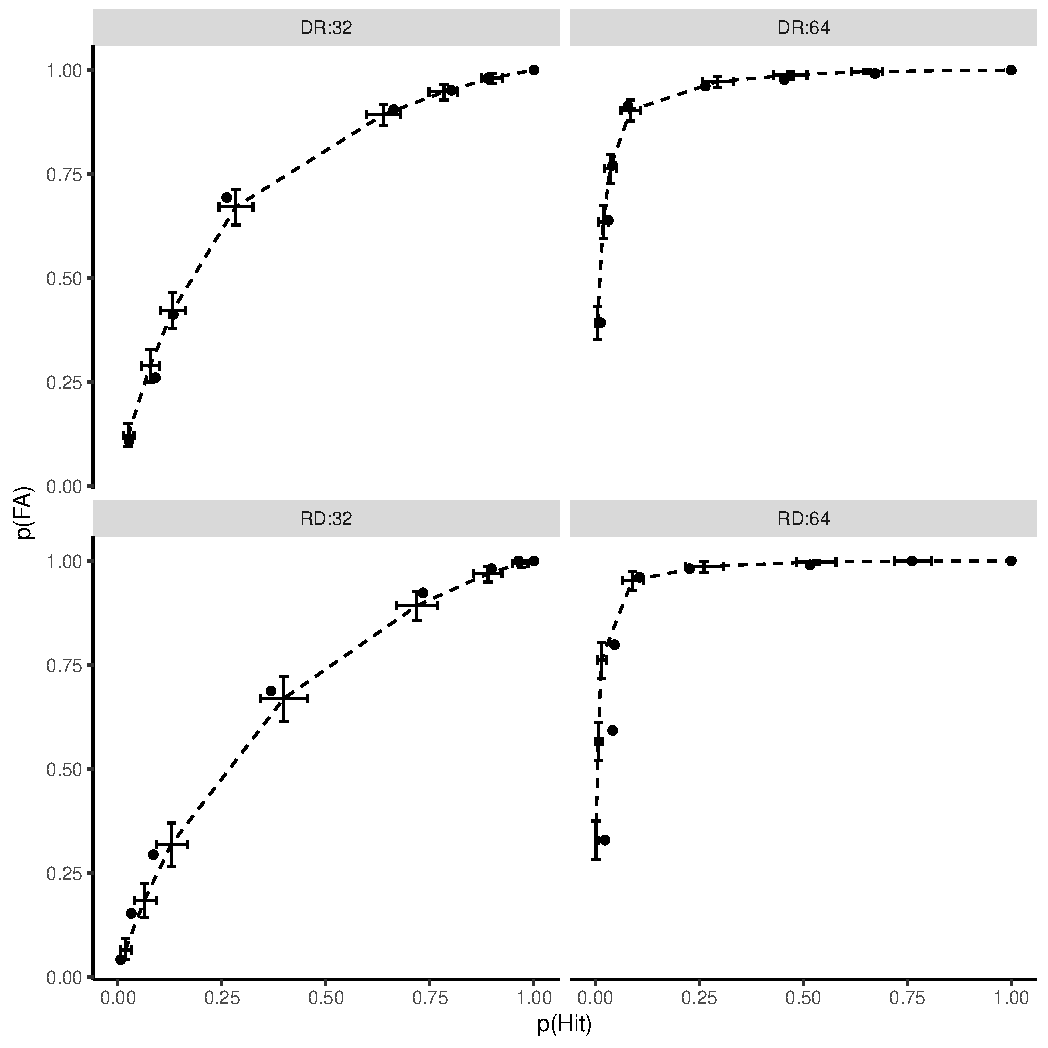
\includegraphics[width=.8\linewidth]{roc_fit.pdf}
  \caption{ROC curve fit}
  \label{fig:3}
\end{figure}

Another way to assess a model fit visually is by inspecting the
% ?? to mają być conditional response distr. dla tego model fita
conditional response distributions ($p(y|stim)$) such as those shown
in Fig.~\ref{fig:4}, which was also created using the
\texttt{plot\_sdt\_fit} function.

\begin{figure}[H]
  \centering
  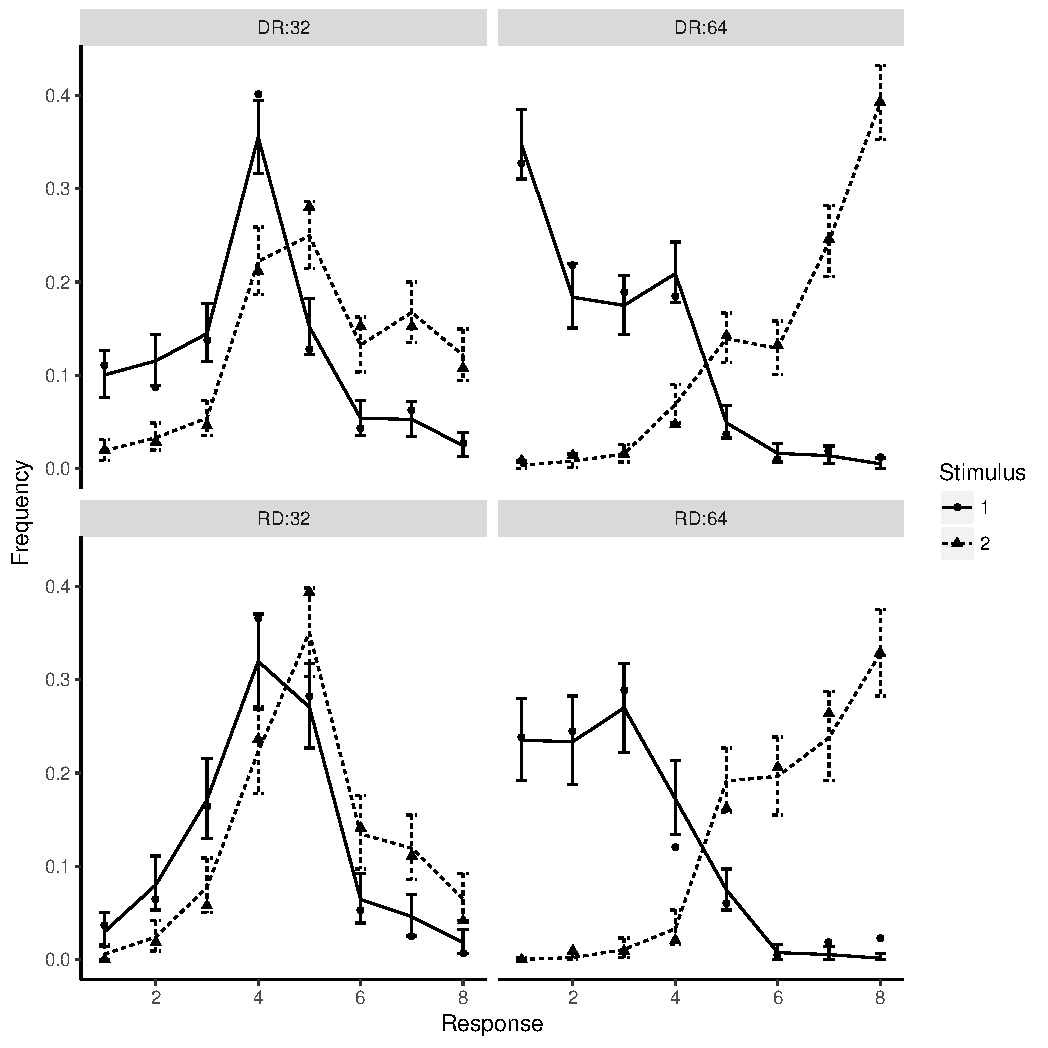
\includegraphics[width=.8\linewidth]{response_fit.pdf}
  \caption{Response distribution fit}
  \label{fig:4}
\end{figure}

% ?? przedimek reasons? niby the model, bo dla plotu model jest już
% określony, ale tu jest this kind of plot
This kind of plot can be informative about the reasons why a model
does not fit the data. In this particular case the plot seems to
suggest that it may be a good idea to inspect the fit at the
individual level and see if there are some participants with unusual
$p(y|stim=1)$ distributions in the RD $\times$ 64 ms condition. On the
other hand, it is also possible that the lack of fit is mainly a
consequence of the assumption that duration had zero effect on
$\bm{\gamma}$, or that more substantial modifications are necessary,
such as dropping the equal variance assumption.

\subsubsection{Converting unconstrained $\delta$ and $\gamma$
  parameters to sensitivities and criteria}

Posterior $\delta$ and $\gamma$ samples have to be transformed in
order to work with the $d'$ and $c$ parameters. This is
straightforward only when fixed effects represent average parameter
values in separate conditions, not differences between conditions or
regression slopes. In our example, because separate intercepts and
slopes parametrization was used for the $\delta$ fixed effects model
matrix, all four \texttt{delta\_fixed} parameters can easily be
transformed to sensitivities by applying the natural logarithm
function. It is important to remember that, because the logarithm is a
non-linear transformation, the $\delta$ to $d'$ conversion step should
be done first, before
% ?? nie wiem czemu the posterior samples, ale tak czuję
applying any other transformations to the posterior samples, for
example, the logarithm of a point and interval $\delta$ estimate is
not equal to the point and interval $d'$ estimate calculated after
transforming the $\delta$ posterior samples to the $d'$ samples.

In this case the first column of the \texttt{gamma\_fixed} parameter
matrix (the intercept) corresponds to the values of the $\bm{\gamma}$
vector in the DR condition but the second column corresponds to the
\emph{effect} of order on $\bm{\gamma}$. For this reason in this
particular case the posterior criteria samples can be obtained using
the \texttt{gamma\_to\_crit} function only for the first column of the
\texttt{gamma\_fixed} matrix.

\subsection{Testing the model on simulated data}

To test if the model correctly recovers known parameter values we have
simulated the data from a hypothetical exact replication of the
previously described experiment using the point estimates from the
previous fit as known realistic parameter values. Mixing performance
was similar to the real data case. All the model parameters were
correctly recovered in a sense that the true values were outside the
95\% credible intervals no more than 5\% of the time.

For illustration purposes an SDT model that differed from the true
model only in that it did not have any hierarchical structure was
fitted to the same simulated dataset. Since the non-hierarchical model
was much simpler and the data consisted of only eight vectors of
response counts the mixing of the chains was excellent.

The 95\% credible intervals calculated for the fixed effects based on
each model are compared in Fig.~\ref{fig:5} below. The estimates were
centered on the true values to simplify the presentation. As can be
seen, the true model correctly recovered the known parameter values,
but the estimates based on the simplified, non-hierarchical model were
biased; the $95\%$ credible intervals were not only about three times
shorter on average but also failed to contain most of the true values.

\begin{figure}[H]
  \centering
  \includegraphics[width=.8\linewidth]{true_vs_nonhier.pdf}
  \caption{Comparison of the point and interval posterior estimates
    based on the true hierarchical and the simplified non-hierarchical
    models}
  \label{fig:5}
\end{figure}

However, as can be seen in Fig.~\ref{fig:8} below in this case the
observed ROC curves seemed to fit the simplified model's predictions
quite well, giving a false impression of model validity.

\begin{figure}[H]
  \centering
  \includegraphics[width=.8\linewidth]{roc_sim_aggr_fit.pdf}
  \caption{ROC curve fit for the non-hierarchical model}
  \label{fig:8}
\end{figure}

\section{Concluding remarks}

The great importance of SDT to psychology stems from the fact that
given weak assumptions about an underlying decision process it
promises to deconfound sensitivity from bias in arbitrary
classification tasks. To the best of our knowledge at present the
\texttt{bhsdtr} package provides the only method of bayesian inference
for SDT models with or without ratings that can be recommended as a
default choice in typical applications. Our parametrization forces the
sensitivity to be non-negative and the criteria to be order-restricted
while the isomorphisms between the $d'$ and $c$ parameters and the
unconstrained $\delta$ and $\gamma$ parameters make it possible to
supplement the SDT model with the general hierarchical linear
regression structure. There is no limit to the number of sampled
factors except for the one imposed by available computational
resources, correlations of random effects of the same sampled factor
are accounted for, all the SDT parameters can be modelled by linear
regression within the same model and all the effects on all the SDT
parameters estimable within the levels of the sampled factors can have
associated random effects. In case a need arises to relax a built-in
restriction experienced users can extend the model in arbitrary ways
by using automatically generated human-readable Stan code as a
% ?? basic understanding niepoliczalne
template. We hope that researchers with basic understanding of Signal
Detection Theory, bayesian inference, and hierarchical modelling will
find our package useful and adopt it as a method of analysis of
classification performance in their future studies.

\bibliography{/home/borys/cs/literatura}
\bibliographystyle{apacite}
\end{document}
